\title{Nektar++ for stability analysis}

\newcommand\gmsh{\emph{Gmsh}~}
\newcommand\nektar{\emph{Nektar++}~}

\documentclass[a4paper,12pt]{article}
\usepackage{tikz}
\usepackage[top=2cm,bottom=3cm,left=1.5cm,right=1.5cm]{geometry}
\usepackage[lined,algo2e,boxed]{algorithm2e}

\setlength{\parindent}{0pt}
\setlength{\parskip}{1ex} 

\begin{document}
\maketitle

The aim of this tutorial is to introduce the user to the spectral/$hp$
element framework \nektar and its use for simple stability analyses of flows. This guide assumes
the user has successfully compiled the libraries, the solvers and the utilities,
as explained on the website\footnote{www.nektar.info}. A series of regression
tests are included to check that the software is producing the expected results.
Please ensure these all pass before continuing.

\textbf{Note}: The example commands given assume the \nektar executables can be
found in your shell path. If you have not set your path accordingly you will
need to specify the full path to the \nektar executable.
\bigskip

In the first section it will be presented the stability analysis of the two dimensional channel flow,
through both the splitting scheme and the Stokes algorithm.\textcolor{red}{ It will be then studied the transient growth
of the flow past a backfacing step and the direct/adjoint stability analysis of a flow past a cylinder.}

\section{Two-dimensional Channel flow}

The linear stability analysis is a technique that allows to determine the asymptotic stability of a given flow.
First of all, let us consider the non-dimensional, viscous linearised Navier-Stokes equations. These equations describe the evolution of an infinitesimal perturbation of the fields for a given base flow.

\begin{equation} \label{perturbationeqns}
\frac{\partial \mathbf{u'}}{\partial t} + \mathbf{U} \cdot \nabla{\mathbf{u'}} + \mathbf{u'} \cdot \nabla{\mathbf{U}}  =-\nabla p' + \frac{1}{Re}\nabla^{2} \mathbf{u'}+\mathbf{f'}
\end{equation}
with continuity equation
\begin{equation}
\nabla \cdot \mathbf{u'}=0
\end{equation}

$\mathbf{u'}$ and $p'$ represent the perturbations of the velocity and pressure, while $\mathbf{U}$ the base flow. 
We will consider as parallel base flow through a 2-D channel (known as Poiseuille flow) at Reynolds number $Re=7500$:

\begin{equation}
\mathbf{U}=y(1-y)\mathbf{e_x}
\end{equation}

The domain is $\Omega=[-\pi,\pi] \times [-1,1]$ and it is composed by 48 quadrilaterals as shown in figure (\ref{Channel_mesh})

\begin{figure}
\centering
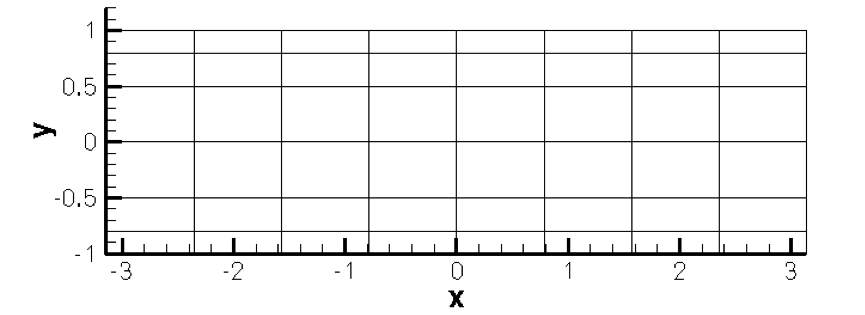
\includegraphics[scale=1]{mesh_chan.png}
\caption{48 quadrilaterals mesh}
\label{Channel_mesh}
\end{figure}

This simple mesh was created using the software $Gmsh$ and the first step is to convert it into a suitable input format so that it can be processed by $Nektar++$ libraries.

\vspace{1cm}
In the tutorial folder \texttt{NekTutorial/Tutorial/Channel/Geometry} you will find the following files: 
\begin{itemize}
\item \texttt{Channel.msh}- $Gmsh$ generated mesh data listing mesh vertices and elements. This is the mesh file used by the $Nektar++$ pre-processing utilities.
\item \texttt{Channel.xml} - \nektar session file generated from
\texttt{Channel.msh} using a \nektar utility. \end{itemize}

\texttt{Channel.xml} can be generated using the \texttt{MeshConvert} pre-processing tool in the \\
\texttt{utilities/builds/PreProcessing/} directory. To generate the $.xml$ file
from the \texttt{.msh} file, run the command

\begin{verbatim}
MeshConvert Channel.msh Channel.xml
\end{verbatim}

\section{Computation of the base flow}

The first step is creating an appropriate base flow that is necessary for solving the the linearised equations. Since in the hydrodynamic instability theory, it is assumed that the base flow is a incompressible, it can be easily computed using the Incompressible Navier-Stokes solver.\\ Moreover, the boundary condition will be no-slipping conditions on the walls and periodic ones for the inflow/outflow. In this case, since  it  is not a constant pressure gradient that drives the flow, it is required to set up a constant body-force in the axial direction that it is easy to verify is equal to $8\nu$. 

\vspace{5mm}

 In the folder \texttt{NekTutorial/Tutorial/Channel/Base}  it is present the file \texttt{Channel-Base.xml} that contains the geometry above described and the necessary parameters to solve the problem.\\
 The \texttt{GEOMETRY} section defines the mesh of the problem and it is generated automatically through the pre-processing utilities. The expansion type and order is specified in the \texttt{EXPANSIONS} section. An expansion basis is applied to a geometry composite specified in the \texttt{GEOMETRY} section. A default entry is always included by the \texttt{MeshConverter}. In this case \texttt{C[0]} refers to the set of all elements. The \texttt{TYPE} tag specifies the choice of the polynomial functions to use in the expansion. It can be set to \texttt{FOURIER} or \texttt{CHEBYSHEV}.  In this case it was chosen to use the \texttt{GLL\_LAGRANGE} that refers to Lagrange polynomials through the Gauss, Lobatto As an alternative, it is possible to use  \texttt{MODIFIED}  that refers to a basis of Legendre polynomials modified to enable the boundary/interior decomposition.The section \texttt{FIELDS} specifies the fields that are considered in the problem, for example the two components of the velocity and the pressure.

\begin{verbatim}
<EXPANSIONS>
    <E COMPOSITE="C[0]" NUMMODES="8"  FIELDS="u,v,p" TYPE="MODIFIED"/>
</EXPANSIONS>
\end{verbatim}

If we examine \texttt{Channel-Base.xml}, we can see how to define the
conditions of the particular problem to solve. These are all enclosed
in a \texttt{CONDITIONS} section. This section contains a number of things:

\begin{enumerate}
\item \textbf{Solver information} (\texttt{SOLVERINFO}) such as the equation type, the projection type
(\texttt{Continuous} or \texttt{Discontinuous} Galerkin), the kind of advection term (\texttt{Convective}, \texttt{Linearised}, \texttt{Adjoint}) and problem to solve (\texttt{Driver} property), along with other properties. The solver properties are specified as quoted
attributes and have the form
\begin{verbatim}
<I PROPERTY="[STRING]" VALUE="[STRING]" />
\end{verbatim}

\textbf{To Do}: In the \texttt{SOLVERINFO} section set the
property \texttt{EQTYPE} to \texttt{UnsteadyNavierStokes}  to select the non-linear incompressible Navier-Stokes equations., the \texttt{ADVECTIONFORM} to \texttt{Convective} and the \texttt{Projection} property to \texttt{Continuous}.   The property \texttt{Driver} selects the type of problem to solve (stability analysis with different methods to compute the eigenvalues or computation of the solution of the 
equations). In this case, set its value to \texttt{STANDARD} to compute and print the solution of the non-linear Navier-Stokes equations.


\item The \textbf{parameters} are specified as name-value pairs:
\begin{verbatim}
<P> [KEY] = [VALUE] </P>
\end{verbatim}
Parameters may be freely used either from within the solver , or within other expressions, such as function definitions or
other parameters defined subsequently.

 \textbf{To Do}: Declare a parameter \texttt{Re} that sets the Reynolds to 7500 and \texttt{Kinvis} equal to $1/Re$ that represents the the kinematic viscosity $\nu$. 


\item The declaration of the variable(s).  
\begin{verbatim}
<VARIABLES>
    <V ID="0"> u </V> 
</VARIABLES>
\end{verbatim}

\item The specification of boundary regions in terms of composites defined in
the geometry and the conditions applied on those boundaries. Boundary regions
have the form
\begin{verbatim}
<B ID="[INDEX]"> [COMPOSITE-ID] </B>
\end{verbatim}


The boundary conditions enforced on a region take the following format for one
or more variable names specified in the \texttt{VARIABLES} section. The
\texttt{REF} attribute for a boundary condition region should correspond to the
\texttt{ID} of the desired \texttt{BOUNDARYREGION}.
\begin{verbatim}
<REGION REF="[B-REGION-INDEX]">
    <[TYPE] VAR="[VARIABLE]" VALUE="[EXPRESSION]"/>
    ...
</REGION>
\end{verbatim}

\item The definition of the forcing term, $f$, and the exact solution. A body-forcing
term has the form
\begin{verbatim}
<FUNCTION NAME="BodyForce">
<E VAR="[VARIABLE]" VALUE="[EXPRESSION]"/>
</FUNCTION>
\end{verbatim}

\textbf{To Do}: Define a body forcing  $f_x=8\nu$ in the axial direction.

\textbf{Todo}: Define the section for the \texttt{EXACTSOLUTION} along with an
expression for $u_{ex}$. The format is identical to that for specifying the
forcing function.
\end{enumerate}

This completes the specification of the problem on the rectangualar mesh.
It can then be solved using the \texttt{IncNavierStokesSolver}.
 The executable is located in the folder
\texttt{solver/builds/dist/bin/}\footnote{If you compiled the library in Debug
mode, the executables will have the suffix \texttt{-g}.}

\begin{verbatim}
IncNavierStokesSolver Channel-Base.xml
\end{verbatim}

To view the output in \gmsh use the post-processing
tools in the \texttt{utilities} directory, as we have done for the
pre-processing. You can produce outputs for \gmsh, $TecPlot$ and $Paraview$
using the corresponding converter from the terminal. For example, to convert the
\texttt{Channel-Base.fld} to \gmsh format, use

\begin{verbatim}
FldToGmsh Channel-Base.xml Channel-Base.fld
\end{verbatim} 


\clearpage
\section{Stability analysis}

After having computed the base flow it is now possible to calculate the eigenvalues and the eigenmodes of the linearised Navier-Stokes equations. Two different algorithm can be used to perform this analysis: the splitting scheme (\texttt{VelocityCorrectionScheme}) and the Stokes algorithm (\texttt{CoupledLinearisedNS}).  We will consider both cases, highlighting the similarities and differences of these two methods. In this tutorial it will be used the Implicitly Arnoldi Method (I.R.A.M.), that is implemented in the open-source $Arpack$ library.

\subsection{Splitting Scheme Method}

The first analysis to run is the computation of the leading eigenvalues and eigenvectors for using the splitting scheme method. It is necessary that the base flow file, computed  in the previous section, is copied in the folder  \texttt{NekTutorial/Tutorial/Channel/VelocityCorrectionScheme} and renamed \texttt{Channel\_VCS.bse}, that is the format used by the code to upload an external flow.  In this folder it is possible to find the file \texttt{Channel\_VCS.xml} that contains all the necessary specifications to perform the direct stability analysis. The format is similar to the one described in the previous section, therefore only the main differences are going to be discussed.

\smallskip
The \texttt{GEOMETRY}, the \texttt{TYPE} and  number of modes (\texttt{NUMMODES}) must be the same used for the base flow, so they are not going to be described again. However, it is important to set some important parameters that are characteristic of the method. 

\textbf{To Do}: 

\begin{enumerate}
\item the \texttt{AdvectionForm} in this case should be set to \texttt{Linearised} in order to select the linearised Navier-Stokes advection term. 
\item \texttt{Driver} must be set to \texttt{Arpack} to use $Arpack$ library .  
\item To start Arnoldi method with a random initial vector it is necessary to add the Solver Info \texttt{InitialVector} to \texttt{Random}.
\item  It can be specified what kind of eigenvalues to compute through the solver property\\ \texttt{ArpackProblemType},
 in particular the ones with the largest magnitude (\texttt{LargestMag}), largest real part (\texttt{LargestReal)} or largest imaginary part (\texttt{LargestIm}). In our case we are interested in computed the eigenvalues with the largest magnitude that determinate the stability of the flow.

\item A series of parameters to make I.R.A.M. work are then specified. 

\begin{itemize}
\item \texttt{kdim}: it is the dimension of Krylov-subspace.
\item \texttt{nvec}: it is the number of requested eigenvalues.
\item \texttt{nits}: it is the number of maximum allowed iterations.
\item \texttt{evtol}: it is the accepted tolerance on the eigenvalues and it determines the stopping criterion.
\end{itemize}

\end{enumerate}
It is now possible to run the direct stability analysis for the channel flow, typing:

\texttt{IncNavierStokesSolver Channel\_VCS.xml}

The code will converge after 264 iterations printing the requested eigenvalues and eigenmodes both on screen on the file \texttt{Channel\_VCS.evl}.

\vspace{0.5cm}
The values printed allow to write the eigenvalues in an exponential form $M e^{i\theta}$ where $M=|\lambda|$ is the magnitude, while $\theta= arctan (\lambda_i/\lambda_r)$.  

\begin{equation}
\lambda_{1,2}= 1.0024 e^{\pm 0.24984 i}
\end{equation}

It is interesting to consider more general quantities that do not depend on the time length of each iteration $T$. For this purpose it was considered the growth rate $\sigma=ln(M)/T$ and the frequency $\omega= \theta/T$. Verify that for this case:

\begin{equation}
\sigma=2.23711 \cdot 10^{-3}
\end{equation}

\begin{equation}
\omega=\pm 2.498413 \cdot 10^{-1}
\end{equation}

This values are in accordance with the literature, in fact in Canuto et al., 1988 suggests $2.23497\cdot 10^{-3}$ and $2.4989154\cdot 10^{-1}$ for growth and frequency respectively.
The eigenmodes associated to the computed eigenvalues are stored in the vectors \texttt{Channel\_VCS\_eig\_1} and \texttt{Channel\_VCS\_eig\_2}. It is then possible to convert this file into a $Gmsh$ output using $Nektar++$ post-processing routines. For the first eigenvector, for example:

\begin{verbatim}
FldToGmsh Channel_VCS.xml Channel_VCS_eig_1
\end{verbatim}

\clearpage
\subsection{Stokes Algorithm}

It is now possible to perform the same stability analysis using a different method base on the Stokes algorithm. This method requires the solution of the full velocity-pressure system, meaning that the velocity matrix system and the pressure system are coupled, differently from the splitting/projection schemes. It is easy to extend this method to solve the unsteady  Navier-Stokes equations introducing  into the Stokes problem an unsteady term $\mathbf{u_f}$ that modifies the weak Laplacian operator into a weak Helmoholtz operator. Furthermore, the non-linear terms are explicitly advanced in time and treated as a forcing function to the Stokes solver.

\vspace{0.5cm}

Inside the folder \texttt{NekTutorial/Tutorial/Channel/CoupledSolver} it is present the file\\ \texttt{Channel\_Coupled.xml} that contains all the necessary parameters that should be defined. Similarly to the previous case, it is possible to specify the base flow putting the \texttt{Channel\_Coupled.bse} in the working directory. However, it is possible to specify the base flow directly from session file if it has an analytical expression like in our example. This second method will the be presented in this section. Even in this case, the geometry, the type and number of modes are the the same of the previous simulations.

\vspace{0.5cm}

\textbf{To Do}: 
\begin{itemize}
\item Set up the \texttt{SolverType} tag to \texttt{CoupledLinearisedNS} in order to solve the linearised Navier-Stokes equations using $Nektar++$'s coupled solver.  
\item the \texttt{EQTYPE} must be set to \texttt{SteadyLinearisedNS} and the \texttt{Driver} to \texttt{Arpack}. 
\item To compute the eigenvalues with the largest magnitude, specify \texttt{LargestMag} in the property \texttt{ArpackProblemType}.
\end{itemize}

It is important to note that the usage of the coupled solver requires that \textbf{only the velocity components} must be specified, while the pressure can be directly computed through their values. 

\vspace{0.5cm}

\textbf{To Do}: In this case it is a body force that provides the driving of the flow. This is done by the setting the  previously introduced function \texttt{BodyForce}  to $cos(y)$ for the $u$ component and $sin(y)$ for the $v$ component.  At last it is necessary to set up the  base flow. In this case, since we have an analytical expression we can define it through the function:

\begin{verbatim}
<FUNCTION NAME="AdvectionVelocity">
<E VAR="[VARIABLE]" VALUE="[EXPRESSION]"/>
</FUNCTION>
\end{verbatim}

The $u$ component must be set up to $1-y^2$, while the $v$-component to zero.\\
It is now possible to run the simulation typing:

\begin{verbatim}
./IncNavierStokesSolver Channel_Coupled.xml
\end{verbatim}

Using the Stokes algorithm, we are computing the leading eigenvalue of the inverse of the evolution operator  $\mathcal{L}^{-1}$\footnote{$\mathcal{L}$ is the evolution operator $d \mathbf{u}/dt=\mathcal{L} \mathbf{u}$}. Therefore the eigenvalues of  $\mathcal{L}$ are the inverse of the found values found. However, it is interesting to note that the value is different from the one calculated with the Splitting Scheme Method, producing an apparent inconsistency in the results. However, this can be explained considering that the largest eigenvalues associated to the operator $\mathcal{L}$ correspond the ones that are clustered near the origin of the complex plane if it is considered the spectrum of $\mathcal{L}^{-1}$. Therefore eigenvalues with a smaller magnitude may be present but they are not associated to the largest magnitude eigenvalue of operator $\mathcal{L}$. In order to verify this issue, it is possible to search the eigenvalues with the largest imaginary part.

\vspace{0.5cm}
\textbf{To Do}: Set up the Solver Info tag \texttt{ArpackProblemType} to \texttt{LargestImag} and run the simulation again.


In this case, it is easy to to see that the eigenvalues of the evolution operator $\mathcal{L}$ are the same ones computed in the previous chapter with the time-stepping approach.

\begin{equation}
\end{equation}
\clearpage


\end{document}
